\documentclass{rithy-thesis}

\title{Thesis Template}
\author{Lim Rithy}
\date{August 2025}

\begin{document}
\pagenumbering{roman} % Set the page number to roman
\chapter*{ACKNOWLEDGMENTS}
\addcontentsline{toc}{chapter}{ACKNOWLEDGEMENTS}

First and foremost, I would like to express my deepest gratitude to \textbf{My Beloved Parents} and \textbf{My Sister}, whose unwavering support, encouragement, and sacrifices have been the foundation of my academic journey. Their love and guidance have continuously motivated me to strive for excellence and overcome every challenge that has come my way. Without their endless support, this achievement would not have been possible.\newline

I would also like to extend my sincere appreciation to \textbf{H.E. Dr. PO Kimtho}, director-general of the Institute of Technology of Cambodia (ITC), for his visionary leadership and dedication to advancing education and research at ITC. His commitment to fostering an environment of academic excellence has provided me with the opportunity to pursue my studies and complete this thesis.\newline

My heartfelt thanks go to \textbf{Dr. CHRIN Phok}, head of the Department of Electrical and Energy Engineering (GEE), and all the professors and lecturers in the department. Their invaluable knowledge, guidance, and dedication to teaching have greatly contributed to my academic and professional development. Their support has played a crucial role in shaping my understanding of electronic and automation engineering.\\

I am profoundly grateful to my advisor, \textbf{Mr. SUM Rithea}, for his invaluable guidance, patience, and encouragement throughout my research. His insightful feedback and unwavering support have been instrumental in shaping the direction of this thesis. Moreover, through working on this thesis and collaborating with him on a research paper, I have gained valuable experience that has enhanced my academic and professional growth.\newline

Finally, I would like to extend my gratitude to my dear friends, \textbf{KEAM Lyvong} and \textbf{KOY Daniel}, for their continuous support, encouragement, and companionship throughout my academic journey. Their friendship has been a source of strength and motivation, making this journey both enjoyable and fulfilling. I am truly grateful to have them by my side.

\chapter*{\khmermuol {សេចក្តីសង្ខេប}}
\addcontentsline{toc}{chapter}{\khmermuol {សេចក្តីសង្ខេប}}

\begin{khmer}
 \hspace{30pt} គោលបំណងចម្បងនៃការសិក្សានេះគឺដើម្បីអនុវត្ត និងប្រើប្រាស់នូវប្រព័ន្ធបញ្ជាផ្អែកលើការ​មើល​ឃើញនិងការកំណត់ សម្រាប់ដៃរ៉ូបូត IRB 1200 ABB ដោយប្រើបច្ចេកទេសក្នុងការសម្គាល់វត្ថុ និងការបញ្ជូនទន្និន័យតាមរយៈទំនាក់ទំនង TCP/IP។ ប្រព័ន្ធមួយនេះត្រូវបានរចនាឡើងដោយប្រើប្រាស់នូវបច្ចេកទេស fine-tuned សម្រាប់កំណត់ និងសម្គាល់វត្ថុ ដែលដំណើរការនៅលើកូដ Python ហើយទទួលរូបភាពបានពីកាម៉េរ៉ានិងគណនាទីតាំងរបស់វត្ថុ។ បច្ចេកទេស projective transformation ត្រូវបានអនុវត្តដើម្បីបំលែងទីតាំងទាំងនេះទៅជាទីតាំងដែលរ៉ូបូតអាចធ្វើបម្លាស់ទីបាន។ ទីតាំងដែលបានគណនាត្រូវបានផ្ញើតាម រយៈទំនាក់ទំនង TCP/IP ទៅកាន់ប្រព័ន្ធបញ្ជារបស់រ៉ូបូត ដើម្បីអនុញ្ញាតឱ្យដៃរ៉ូបូតអាចធ្វើការចាប់យកវត្ថុដោយមានភាពត្រឹមត្រូវនៅក្នុងមជ្ឍដ្ឋាននិមិត្ត។ ការសិក្សានេះផ្តោតតែលើការបញ្ជាទីតាំង ដោយមិនរាប់បញ្ចូលចលនាស៊ីនេម៉ាទិច, ការគ្រប់គ្រងគន្លង, ឬការប្រើប្រាស់ PID សម្រាប់ប្រព័ន្ធបញ្ជា។
\end{khmer}

\chapter*{ABSTRACT}
\addcontentsline{toc}{chapter}{ABSTRACT}

The main objective of this thesis is to implement a system integration and vision-based control system for the IRB 1200 ABB Robot Arm using real-time object detection and TCP/IP communication. The system employs a fine-tuned object detection model running on a Python-based framework to identify custom objects from webcam images and determine their positions in the camera frame. A projective transformation technique is applied to convert these positions into the robot’s coordinate system. The mapped coordinates are then transmitted via TCP/IP to the robot controller, enabling precise object manipulation in a simulated environment. This study focuses solely on position-based control, without incorporating inverse kinematics, trajectory planning, or PID-based motion control. \\

To evaluate system performance, experiments are conducted using a real webcam and a simulated robot environment in RobotStudio. The setup includes workspace calibration and coordinate alignment between the vision system and the robot. System performance is assessed in terms of accuracy, consistency, and overall reliability in detecting and mapping object positions. Challenges such as perspective distortion, coordinate transformation accuracy, and occasional misclassification are considered to identify system limitations and areas for improvement. \\

The findings of this research highlight the feasibility of using a vision-guided approach for robotic control in industrial applications. The results show that integrating object detection with position-based control can effectively guide a robotic arm for automated tasks. This study contributes to the development of efficient and flexible robotic systems and provides a foundation for future enhancements in vision-based automation, especially in dynamic or semi-structured environments.

\chapter*{ABBREVIATIONS}
\addcontentsline{toc}{chapter}{ABBREVIATIONS}

\noindent
\begin{tabular}{l @{\hspace{60pt}} p{0.5\linewidth} r}
\textbf{YOLO} & You Only Look Once & \\
\textbf{PCB} & Printed Circuit Board & \\
\textbf{TCP} & Tool Center Point & \\
\textbf{SVD} & Singular Value Decomposition & \\
\textbf{LAN} & Local Area Network & \\
\textbf{IP} & Internet Protocol & \\
\textbf{API} & Application Programming Interface & \\
\textbf{mAP} & Mean Average Precision & \\
\textbf{$h_{11}, \ldots, h_{33}$} & Elements of homography matrix $H$ & \\
\textbf{$\mathbf{p}$} & Source point vector & \\
\textbf{$\mathbf{p'}$} & Destination point vector & \\
\textbf{$w$} & Source plane scale factor,& \\
\textbf{$w'$} & Destination plane scale factor & \\
\textbf{$x, y$} & Source plane coordinates (pixels) & \\
\textbf{$x', y'$} & Destination plane coordinates & \\
\textbf{$x_c, y_c$} & Bounding box center coordinates & \\
\textbf{$x_{rob}, y_{rob}$} & Robot frame coordinates & \\
\textbf{$x_{tran}, y_{tran}$} & Transformed frame coordinates & \\
\textbf{$z_{wb}$} & Whiteboard z-coordinate,& \\
\textbf{$z_{sp}$} & Sorting position z-coordinate & \\
\end{tabular}

\startcontent


\pagenumbering{arabic} % Set the page number to roman
\spacing{1.5} % ITC Format Spacing

\chapter{INTRODUCTION}
\section{Study Background}
The history of robotic arms dates back to 1495, when \textbf{Leonardo da Vinci} designed a mechanical knight, an early concept of automation. In 1937/38, \textbf{Westinghouse} introduced, a humanoid robot capable of basic speech and movement, showcasing early automation capabilities. The first true industrial robotic arm, was created in 1961 by \textbf{George Devol} and \textbf{Joseph Engelberger}, marking a significant breakthrough in industrial robotics. Installed at \textbf{General Motors (GM)}, Unimate performed hazardous tasks such as lifting and stacking hot die-cast metal parts, improving efficiency and workplace safety. This innovation paved the way for the widespread adoption of robotic arms in manufacturing \cite{moran2007evolution} and the development of more advanced robotic systems in subsequent decades as shown in Figure 1.1.
\begin{figure}[H]
    \centering
    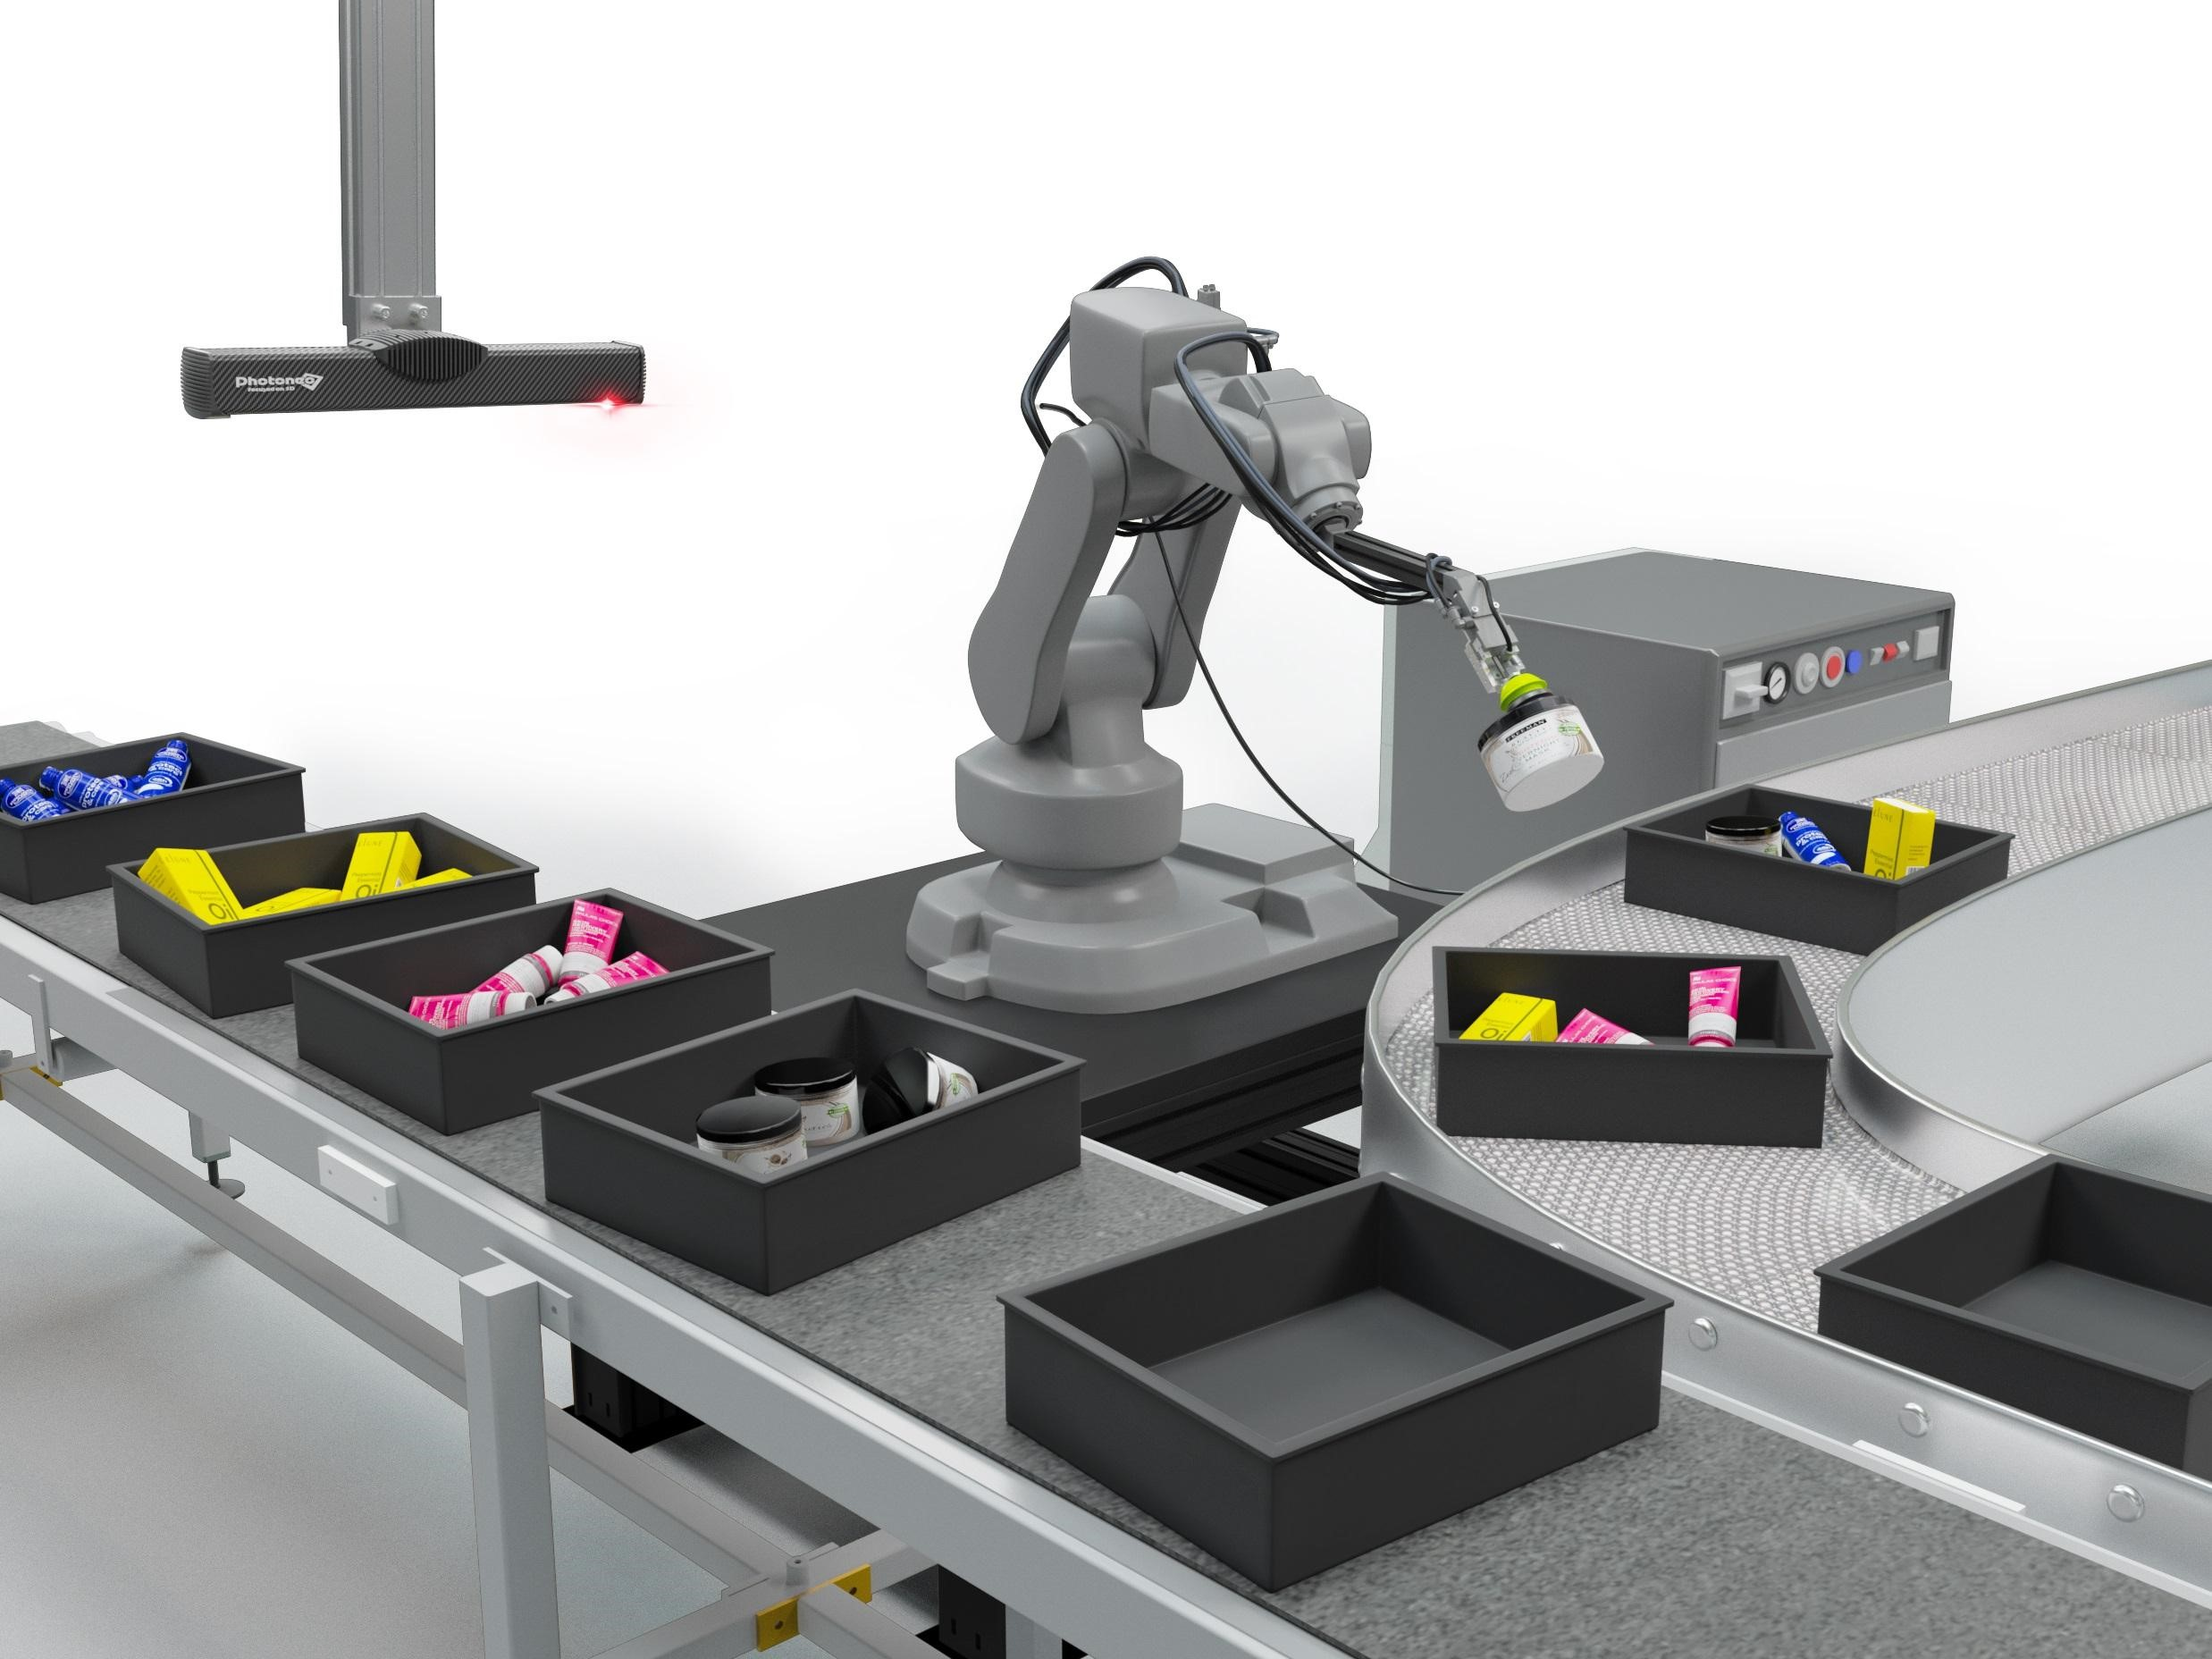
\includegraphics[width=0.75\linewidth]{figures/robotic arm.png}
    \caption{Implementing a camera with a robotic arm for object detection}
    \label{tab:robotic-arm}
\end{figure}

\chapter{LITERATURE REVIEW}
\section{Homography Transformation-based Projective Transformation}

\begin{figure}[H]
    \centering
    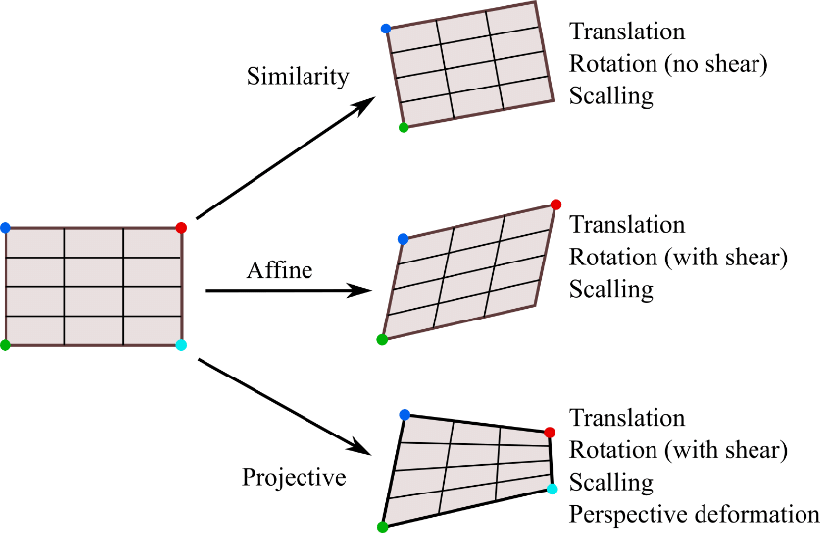
\includegraphics[width=0.75\linewidth]{figures/projective transform.png}
    \caption{Enter Caption}
    \label{fig:placeholder}
\end{figure}
\begin{figure}[H]
    \centering
    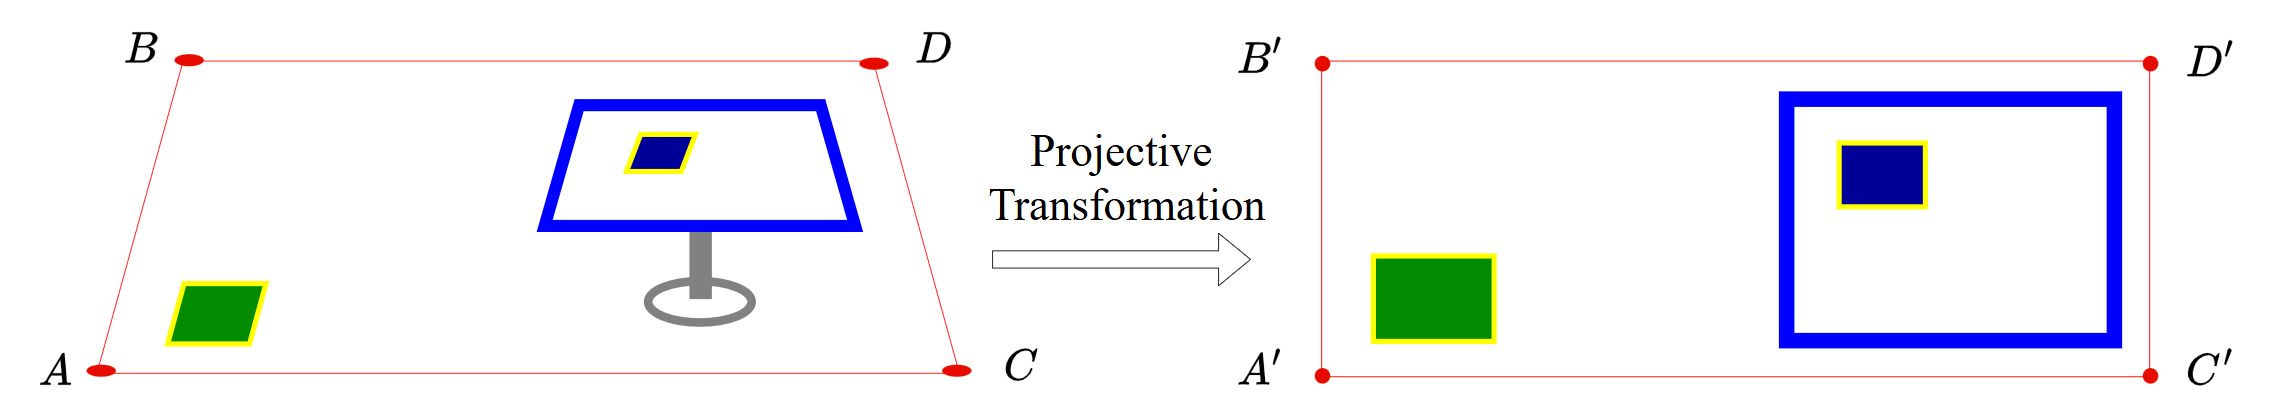
\includegraphics[width=1\linewidth]{figures/transformation.png}
    \caption{Enter Caption}
    \label{fig:placeholder}
\end{figure}

\begin{table}[H]
\renewcommand{\arraystretch}{1.25} % Stretch rows vertically by 1.5x 
\centering
\caption{YOLOv11n Training Summary and Evaluation Results}
\label{tab:param tran}
\begin{tabular}{|l|c|}
\hline
\textbf{Model Summary} & \textbf{Value} \\
\hline
Model Architecture     & YOLOv11n \\
Number of Layers       & 100 \\
Total Parameters       & 2,582,542 \\
\hline
\end{tabular}

\vspace{0.5cm}

\begin{tabular}{|l|c|c|c|c|c|}
\hline
\textbf{Class} & \textbf{Images} & \textbf{Instances} & \textbf{Precision (P)} & \textbf{Recall (R)} & \textbf{mAP@0.5:0.95} \\
\hline
All      & 15 & 22 & 0.976 & 0.997 & 0.877 \\
PCB A    & 12 & 12 & 1.000 & 0.994 & 0.883 \\
PCB B    & 10 & 10 & 0.952 & 1.000 & 0.871 \\
\hline
\end{tabular}
\end{table}

The goal is to obtain the mapped or transformed coordinates, as illustrated in \autoref{fig:map}. To accurately perform a projective transformation, calibration coordinates are essential for solving the projective transformation equations. The parameters used in this process are as follows:
\begin{itemize}
\setlength{\itemsep}{0pt}
\item $A(x, y), B(x, y), C(x, y), D(x, y)$: Coordinates on the source plane.
\item $A'(x, y), B'(x, y), C'(x, y), D'(x, y)$: Corresponding coordinates on the destination plane.
\end{itemize}
The coordinates mentioned above correspond to pixel positions within the captured image frame and are extracted using OpenCV's image processing capabilities. To map these image points to real-world coordinates or to another perspective, a projective transformation is required. Among the available techniques, Homography Transformation is the most commonly used approach due to its effectiveness in handling planar surfaces and perspective distortion. So the Homography Transformation's equation is following:
\begin{align}
    &\mathbf{p'} = H \cdot \mathbf{p}  \label{eq: projective}
\end{align}

where $\mathbf{p'}$ is denoted as the destination plan, $\mathbf{p}$ is denoted as source plan, and $H$ is is the homography matrix that $\in \mathbb{R}^{3 \times 3}$ and following:
\begin{equation}
H = 
    \begin{bmatrix}
    h_{11} & h_{12} & h_{13} \\
    h_{21} & h_{22} & h_{23} \\
    h_{31} & h_{32} & h_{33}
    \end{bmatrix}
    \label{homo}
\end{equation}
% \\
%     &\mathbf{p'} 
%     =
%     \begin{bmatrix}
%     h_{11} & h_{12} & h_{13} \\
%     h_{21} & h_{22} & h_{23} \\
%     h_{31} & h_{32} & h_{33}
%     \end{bmatrix}
%     \cdot
%     \mathbf{p}


% So by using Homography Transformation's theory, we have do a transformation from 2D plan of $P(x,y)$ to 3D plan $\tilde{P}(\tilde{x}, \tilde{y}, \tilde{z})$ that contain the equivalent equation followng:

So, to define Homogeneous coordinates $(h_{11},h_{12},\dots , h_{33})$ from Cartesian coordinates, one more dimension is added as following:

\begin{align}
&\underbrace{
  \begin{bmatrix}
    x \\
    y \\
  \end{bmatrix}
}_{\text{\scriptsize Cartesian coordinates}}
\qquad&\longrightarrow\qquad
\underbrace{
  \begin{bmatrix}
    wx \\
    wy \\
    w
  \end{bmatrix}
}_{\text{\scriptsize Homogeneous coordinates}}
\qquad (w \neq 0) \label{eq:cat2hom}
\end{align}
\begin{align}
&\underbrace{
  \begin{bmatrix}
    wx \\
    wy \\
    w
  \end{bmatrix}
}_{\text{\scriptsize Homogeneous coordinates}}
\qquad&\longrightarrow\qquad
\underbrace{
  \begin{bmatrix}
    \dfrac{wx}{w} \\[1ex]
    \dfrac{wy}{w} \\[1ex]
  \end{bmatrix}
}_{\text{\scriptsize Cartesian coordinates}}
\hspace{1.3cm} (w \neq 0) \label{eq:hom2cat}
\end{align}

As given in \eqref{eq:cat2hom} and \eqref{eq:hom2cat}, those equation above are transformation and reverse transformation between Cartesian coordinates and Homogeneous coordinates, where $x,y$ are coordinate axis of the plan, and $w$ is denoted as scale factor and it can't be equal to 0.\\

Base on this equation, the commonly used value of $w$ is 1. So, the combine equation from the relationship of \eqref{eq: projective}, \eqref{homo}, and \eqref{eq:cat2hom} with new homogeneous factor $w'$ by following:
\begin{equation}
    \begin{bmatrix}
        w'x' \\
        w'y' \\
        w'
    \end{bmatrix}
    =
    \begin{bmatrix}
    h_{11} & h_{12} & h_{13} \\
    h_{21} & h_{22} & h_{23} \\
    h_{31} & h_{32} & h_{33}
    \end{bmatrix}
    \cdot
    \begin{bmatrix}
        x \\
        y \\
        1
    \end{bmatrix}
    \label{eq:matrix homo}
\end{equation}

\noindent For easily, let $\tilde{X} = w'x'$ and $\tilde{Y} = w'y'$. Then the matrix extraction of \eqref{eq:matrix homo} is following:
\begin{align}
    \tilde{X} &= h_{11}x+h_{12}y+h_{13} \label{x}\\
    \tilde{Y} &= h_{21}x+h_{22}y+h_{23} \label{y}\\
    w' &= h_{31}x+h_{32}y+h_{33} \label{eq:w'}
\end{align}

\noindent Since $x' = \frac{\tilde{X}}{w'}$, $y' = \frac{\tilde{Y}}{w'}$, and by applying \eqref{eq:w'} to \eqref{x} and \eqref{y}, then the Cartesian coordinates of destination plan are:
\begin{align}
    x' = \dfrac{h_{11}x+h_{12}y+h_{13}}{h_{31}x+h_{32}y+h_{33}} \Longleftrightarrow x'(h_{31}x+h_{32}y+h_{33}) - h_{11}x+h_{12}y+h_{13} = 0 \\
    y' = \dfrac{h_{21}x+h_{22}y+h_{23}}{h_{31}x+h_{32}y+h_{33}} \Longleftrightarrow y'(h_{31}x+h_{32}y+h_{33}) - h_{21}x+h_{22}y+h_{23} = 0
\end{align}
\noindent Rewriting these into a matrix form leads to the system:
\begin{align}
    \begin{bmatrix}
x & y & 1 & 0 & 0 & 0 & -x' x & -x' y & -x' \\
0 & 0 & 0 & x & y & 1 & -y' x & -y' y & -y'
\end{bmatrix}
\cdot
\begin{bmatrix}
h_{11} \\
h_{12} \\
h_{13} \\
h_{21} \\
h_{22} \\
h_{23} \\
h_{31} \\
h_{32} \\
h_{33}
\end{bmatrix}
=
\begin{bmatrix}
0 \\
0
\end{bmatrix}
\label{ahx}
\end{align}
The homogeneous coordinates \((h_{11}, h_{12}, \dots, h_{33})\) in \eqref{ahx} are computed through calibration by mapping pixel points between the source and destination planes, as shown in \autoref{fig:map}, using the format below:
\begin{equation}
    A\cdot h= 0
\end{equation}

\noindent Where, $h \neq 0$ and we want $Ah$ to be close to 0 as possible. Moreover, if we apply all the relevant parameter of calibration point to $A$, so $A$ have to be $8\times9$ matrix. Then, equation can then be solved using SVD, hence $A$ can be solve by following full SVD:
\begin{equation}
   A = U \Sigma V^{T}
\end{equation}
Where,
\begin{itemize}
\setlength{\itemsep}{0pt}
    \item $U$ $\in$ $\mathbb{R}^{8\times8}$ is orthogonal matrix 8 × 8 shape
    \item $\Sigma$ $\in$ $\mathbb{R}^{8\times9}$ is diagonal matrix 8 × 9, consisting of only non-negative values
    \item $V^{T}$ $\in$ $\mathbb{R}^{9\times9}$ is another orthogonal matrix with 9 × 9 shape.
\end{itemize}
Thus, the substitution of the SVD into the equation is following:
\begin{equation}
    U\Sigma V^{T}\cdot h = 0
\end{equation}


\renewcommand\bibname{REFERENCES}
\bibliographystyle{ieeetr}
\bibliography{bibliography}
\addcontentsline{toc}{chapter}{{REFERENCES}}


\end{document}
